\documentclass[a4paper]{article}
\usepackage[margin=2cm]{geometry}

\def\pgfsysdriver{pgfsys-pdftex.def}

\usepackage{fontspec}
\usepackage[english]{babel} % Language 
\usepackage{enumitem}
\usepackage{listings}
\usepackage[dvipsnames]{xcolor}
\usepackage{graphicx}
\usepackage{float}
\usepackage[hidelinks]{hyperref}
\usepackage{tikz}
\usepackage{pgfplots}
\usepackage[dvipsnames]{xcolor}
\usepackage{multirow}
\usepackage{caption}

\setlength{\parindent}{0pt}
\setlength{\parskip}{1em}

\lstset{
	basicstyle=\ttfamily,
	showspaces=false,
	showstringspaces=false,
	tabsize=4,
	stringstyle=\color{orange},
	commentstyle=\color{OliveGreen},
	keywordstyle=\color{blue},
	numberstyle=\color{Gray}
}

\title{
	\textsc{PAR: Laboratory 1} \\
	\texttt{\large par4201}
}

\author{Joan Marcè i Igual \and Esteve Tarragó i Sanchís}


\begin{document}

\maketitle
\tableofcontents
\pagebreak

\section{OpenMP questionnaire}

When answering to the questions in this questionnaire, please DO NOT simply answer with yes, no or a number; try to minimally justify all your answers. Sometimes you may need to execute several times in order to see the effect of data races in the parallel execution.

\subsection{Basics}

\subsubsection{\texttt{1.hello.c}}

\begin{enumerate}
	\item \textbf{How many times will you see the \texttt{"Hello world!"} message if the program is executed with \texttt{"./1.hello"}?}
\end{enumerate}

We will se 24 times \texttt{"Hello world!"}, one for each thread.

\begin{enumerate}[resume]
	\item \textbf{Without changing the program, how to make it to print 4 times the \texttt{"Hello World!"} message?}
\end{enumerate}

Adding the following environment variable:

\verb|export OMP_NUM_THREADS=4|

\subsubsection{\texttt{2.hello.c}}

\begin{enumerate}
	\item \textbf{Is the execution of the program correct? (i.e., prints a sequence of \texttt{"(Thid) Hello (Thid) world!"} being \texttt{Thid} the thread identifier). Which data sharing clause should be added to make it correct?}
\end{enumerate}

No, the execution is not correct because the variable \verb|id| is global and gets overwritten by each thread.

\begin{enumerate}[resume]
	\item \textbf{Are the lines always printed in the same order? Could the messages appear intermixed?}
\end{enumerate}

No because the thread execution is not sequential and between two \verb|printf| calls from one thread another one can make its \verb|printf| call.

\subsubsection{\texttt{3.how\_many.c}}

\begin{enumerate}
	\item \textbf{How many \texttt{"Hello world ..."} lines are printed on the screen?}
\end{enumerate}

\begin{lstlisting}[language=C]
//8 times
#pragma omp parallel
printf("Hello world from the first parallel!\n");

omp_set_num_threads(2);

//2 times
#pragma omp parallel
printf("Hello world from the second parallel!\n");

//3 times
#pragma omp parallel num_threads(3)
printf("Hello world from the third parallel!\n");

//2 times
#pragma omp parallel
printf("Hello world from the fourth  parallel!\n");

srand(time(0));

//1 time
#pragma omp parallel num_threads(rand()%4+1) if(0) 
printf("Hello world from the fifth parallel!\n");

// Total: 16 times
\end{lstlisting}

\begin{enumerate}[resume]
	\item \textbf{If the \texttt{if(0)} clause is commented in the last parallel directive, how many \texttt{"Hello world ..."} lines are printed on the screen?}
\end{enumerate}

If the \verb|if(0)| is removed then the last directive:
\begin{lstlisting}[language=C]
#pragma omp parallel num_threads(rand()%4+1) 
printf("Hello world from the fifth parallel!\n");
\end{lstlisting}

will print between 1 and 4 lines so the number of lines printed will be
between 16 and 19 lines.

\subsubsection{\texttt{4.data\_sharing.c}}

\begin{enumerate}
	\item \textbf{Which is the value of variable \texttt{x} after the execution of each parallel region with different data-sharing attribute (\texttt{shared}, \texttt{private} and \texttt{firstprivate})?}
\end{enumerate}

\begin{lstlisting}[language=C]
omp_set_num_threads(8);

int x = 0;
#pragma omp parallel shared(x)
{
	x++;
}
// Normally 8 but it may change if there are collisions
printf("After first parallel (shared) x is: %d\n",x);

x = 0;
#pragma omp parallel private(x)
{	 
	x++;
}
// Always 0 since each thread does not modify 
// the x outside its code
printf("After second parallel (private) x is: %d\n",x);

x = 0;
#pragma omp parallel firstprivate(x)
{
	x++;
}
// Always 0 since each thread does not modify 
// the x outside its code too
printf("After third  parallel (first private) x is: %d\n",x);
\end{lstlisting}

\begin{enumerate}[resume]
	\item \textbf{What needs to be changed/added/removed in the first directive to ensure taht the value after the first parallel is always 8?}
\end{enumerate}

The following line needs to be changed:
\begin{lstlisting}[language=C]
#pragma omp parallel shared(x)
\end{lstlisting}

to the following value:
\begin{lstlisting}[language=C]
#pragma omp parallel reduction(+:x)
\end{lstlisting}

\subsubsection{\texttt{5.parallel.c}}
\begin{enumerate}
	\item \textbf{How many messages the program prints? Which iterations is each thread executing?}
\end{enumerate}

The number of messages depends on the trace execution. The iteration each thread is executing depends on the trace too. This is caused because the \verb|i| variable is shared between all the threads.

\begin{enumerate}[resume]
	\item \textbf{What needs to be changed in the directive to ensure that each thread executes the appropriate iterations?}
\end{enumerate}

The following line needs to be changed:
\begin{lstlisting}[language=C]
#pragma omp parallel num_threads(NUM_THREADS)
\end{lstlisting}

to the following value:
\begin{lstlisting}[language=C]
#pragma omp parallel private(i) num_threads(NUM_THREADS)
\end{lstlisting}

\subsubsection{\texttt{6.datarace.c}}
\begin{enumerate}
	\item \textbf{Is the program always executing correctly?}
\end{enumerate}

No, sometimes the execution fails because \verb|x| is not equal to \verb|N| due to the variable being shared.

\begin{enumerate}[resume]
	\item \textbf{Add two alternative directive to make it correct. Which are these directives?}
\end{enumerate}

\begin{enumerate}[label=\roman*)]
	\item Change the following line:
	\begin{lstlisting}[language=C]
#pragma omp parallel private(i)
	\end{lstlisting}
	
	to the following value:
	\begin{lstlisting}[language=C]
#pragma omp parallel private(i) reduction(+:x)
	\end{lstlisting}
	
	\item The second option is to make a part of the code atomic by adding:
	\begin{lstlisting}[language=C]
#pragma omp atomic
x++;
	\end{lstlisting}
\end{enumerate}

\subsubsection{\texttt{7.barrier.c}}

\begin{enumerate}
	\item \textbf{Can you predict the sequence of messages in this program? Do threads exit from the barrier in any specific order?}
\end{enumerate}

The order of the first 4 messages can't be predicted because all the threads are active and there's no way to tell which will be the first to print a message.

After that, the thread with \verb|id = 0| will print \verb|"(0) wakes up and enters barrier..."| and then all the threads ordered by \verb|id| will print this message until all threads are awake.

Finally all threads will print \verb|(x) We are all awake!"| in an undeterministic order since all the threads are active.

\subsection{Worksharing}
\subsubsection{\texttt{1.for.c}}

\begin{enumerate}
	\item \textbf{How many iterations from the first loop are executed by each thread?}
\end{enumerate}

Each thread executes 2 iterations since the compiler distributes the 16 iterations statically between the 8 threads.

\begin{enumerate}[resume]
	\item \textbf{How many iterations from the second loop are executed by each thread?}
\end{enumerate}

The first 3 threads execute 3 iterations and the other threads execute 2 iterations each one. This is because now there are 19 iterations and \verb|OpenMP| distributes this iterations between the 8 threads too.

\begin{enumerate}[resume]
	\item \textbf{Which directive should be added so that the first \texttt{printf} is executed only once by the first thread that finds it?}
\end{enumerate}

The following line needs to be added:
\begin{lstlisting}[language=C]
#pragma omp single
\end{lstlisting}
This directive tells to only one thread execute this code.

\subsubsection{\texttt{2.schedule.c}}

\begin{enumerate}
	\item \textbf{Which iterations of the loops are executed by each thread for each \texttt{schedule} kind?}
\end{enumerate}

\begin{lstlisting}[language=C]
// Each thread executes 4 consecutive iterations
#pragma omp for schedule(static)

// Each thread executes 2 chunks of 2 consecutive iterations
#pragma omp for schedule(static, 2)

// Each thread executes chunks of 2 iterations and then requests 
// another chunk. So the number of thread iterations depends 
// in the execution.
#pragma omp for schedule(dynamic,2)


// Each thread executes chunks of at least 2 iterations and 
// then requests another chunk. The number of thread iterations 
// depends in the execution too.
#pragma omp for schedule(guided,2)
\end{lstlisting}

\subsubsection{\texttt{3.nowait.c}}

\begin{enumerate}
	\item \textbf{How does the sequence of \texttt{printf} change if \texttt{nowait} clause is removed from the first \texttt{for} directive?}
\end{enumerate}

The second loop is never executed before all threads have finished the first loop. This causes that all the \verb|Loop 1| mesages are printed before all the \verb|Loop 2| messages.

\begin{enumerate}[resume]
	\item \textbf{If the \texttt{nowait} clause is removed in the seconde \texttt{for} directive, will you observe any difference?}
\end{enumerate}

No it won't since after the \verb|parallel| directive finishes all threads wait to syncronize.

\subsubsection{\texttt{4.collapse.c}}
\begin{enumerate}
	\item \textbf{Which iterations of the loop are executed by each thread when the \texttt{collapse} clause is used?}
\end{enumerate}

\begin{table}[H]
	\centering
	\begin{tabular}{crr}
		Thread ID & \verb|i| & \verb|j| \\
		\hline
		\multirow{4}{*}{0} & 0 & 0 \\
		& 0 & 1 \\
		& 0 & 2 \\
		& 0 & 3 \\
		\hline
		\multirow{3}{*}{1} & 0 & 4 \\
		& 1 & 0 \\
		& 1 & 1 \\
		\hline
		\multirow{3}{*}{2} & 1 & 2 \\
		& 1 & 3 \\
		& 1 & 4 \\
		\hline
		\multirow{3}{*}{3} & 2 & 0 \\
		& 2 & 1 \\
		& 2 & 2 \\
		\hline
		\multirow{3}{*}{4} & 2 & 3 \\
		& 2 & 4 \\
		& 3 & 0 \\
		\hline
		\multirow{3}{*}{5} & 3 & 1 \\
		& 3 & 2 \\
		& 3 & 3 \\
		\hline
		\multirow{3}{*}{6} & 3 & 4 \\
		& 4 & 0 \\
		& 4 & 1 \\
		\hline
		\multirow{3}{*}{7} & 4 & 2 \\
		& 4 & 3 \\
		& 4 & 4 \\
	\end{tabular}
\end{table}

\begin{enumerate}[resume]
	\item \textbf{Is the execution correct if the \texttt{collapse} clause is removed? Which clause (different than \texttt{collapse}) should be added to make it correct?}
\end{enumerate}

No, the execution is not correct because the variable \verb|j| becomes shared and there will be conflicts.

To make it correct then the following clause needs to be added before the nested \verb|for|:

\begin{lstlisting}[language=C]
#pragma omp parallel for
\end{lstlisting}

\subsection{Tasks}
\subsubsection{\texttt{1.serial.c}}

\begin{enumerate}
	\item \textbf{Is the code printing what you expect? Is it executing in parallel?}
\end{enumerate}

The code is printing what I expect but it's not executing in parallel because all the tasks are done in thread 0.

\subsubsection{\texttt{2.parallel.c}}
\begin{enumerate}
	\item \textbf{Is the code printing what you expect? What is wrong with it?}
\end{enumerate}

The code is not printing what I expect because is not computing properly the Fibonacci number. 

\begin{enumerate}[resume]
	\item \textbf{Which directive should be added to make its execution correct?}
\end{enumerate}

After the following line:
\begin{lstlisting}[language=C]
#pragma omp parallel firstprivate(p) num_threads(4)
\end{lstlisting}

The following clause must be added:
\begin{lstlisting}[language=C]
#pragma omp single
\end{lstlisting}

\begin{enumerate}[resume]
	\item \textbf{What would happen if the \texttt{firstprivate} clause is removed from the task directive? And if the \texttt{firstprivate} clause is ALSO removed from the \texttt{parallel} directive? Why are they redundant?}
\end{enumerate}

If we remove the \texttt{firstprivate} from the task directive the code works but if we remove the \texttt{firstprivate} from the parallel directive too then a segmentation fault is produced. 

They are redundant because if you add \texttt{firstprivate} in the parallel directive by default the task directive adds the \texttt{firstprivate} option too.

\begin{enumerate}[resume]
	\item \textbf{Why the program breaks when variable \texttt{p} is not \texttt{firstprivate} to the task?}
\end{enumerate}

In the last iteration of the loop there are still threads doing the work but the thread controlling the while loop sets p to null and the other threads try to access to a null pointer.

\begin{enumerate}[resume]
	\item \textbf{Why the \texttt{firstprivate} clause was not needed in \texttt{1.serial.c}?}
\end{enumerate}

Because there was only one thread and there was no possible conflicts between different threads.

\section{Parallelization overheads}

\begin{enumerate}
	\item \textbf{Which is the order of magnitude for the overhead associated with \texttt{parallel} region(fork and join) in \texttt{OpenMP}? Is it constant? Reason the answer based on the results reported by the \texttt{pi\_omp\_overhead.c} code.}
\end{enumerate}

The overhead time is about 0,2 microseconds of the execution time and tends to be constant by thread. If we increase the number of threads the total overhead increases too.

\begin{enumerate}[resume]
	\item \textbf{Which is the order of magnitude for the overhead associated with the execution of \texttt{critical} regions in \texttt{OpenMP}? How is this overhead decomposed? How and why does the overhead associated with \texttt{critical} increase with the number of processors? Identify at least three reasons that justify the observed performance degradation. Base your answers on the execution times reported by the \texttt{pi\_omp.c} and \texttt{pi\_omp\_critical.c} programs and their \texttt{Paraver} execution traces.}
\end{enumerate}

The order of magnitude is about 2 s per thread per 100 000 000 iterations. 

There is a lot of overhead due to the critical region. With one thread the seq time was 0.79s compared to the critical one that was 1.83s for making the same task (so 1.04s of overhead 57% of the time).  

With 8 threads the total time increased a lot in the critical program, it was 22.94 s which shows that the overhead increase with the number of threads. We would expect the program to run in less time with more threads but happens the opposite way due to overhead.

The sequential code does not benefit from the increment of threads and it’s time remains the same.

The overhead time is increasing more than linary cause the overhead per thread increased when the number of processor increased. That’s caused by synchronization among threads.


\begin{table}[H]
    \centering
    \begin{tabular}{l|rrrr}
        \parbox{2.5cm}{100.000.000 iterations times} & \verb|Seq| & \verb|Critical| & Overhead & \parbox{2cm}{\raggedleft Overhead per thread} \\
        \hline
        1 thread & 0,79 & 1,83 & 1,04 & 1,04 \\
        8 threads & 0,79 & 22,94 & 22,15 & 2,77
    \end{tabular}
\end{table}

The following images show \verb|paraver| results under 100.000 iterations with \verb|pi_omp_critical| with one and eight threads.

\begin{figure}[H]
    \centering
    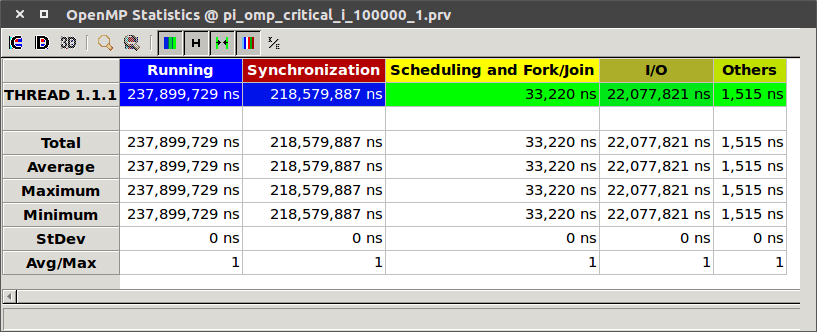
\includegraphics[width=0.9\textwidth]{images/image00}
    \caption{Lock with 1 thread}
    \label{fig:image00}
\end{figure}

\begin{figure}[H]
    \centering
    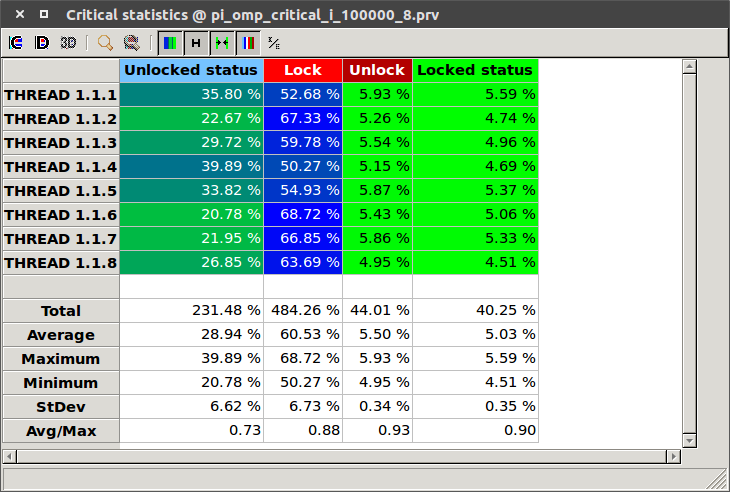
\includegraphics[width=0.8\textwidth]{images/image01}
    \caption{Lock with 8 threads}
    \label{fig:image01}
\end{figure}

\autoref{fig:image00} and \autoref{fig:image01} images show us the the percentage of the time that threads are locked. As we were expecting the executions with 8 threads has a lower unlocked time than the one with 1 thread.

\begin{figure}[H]
    \centering
    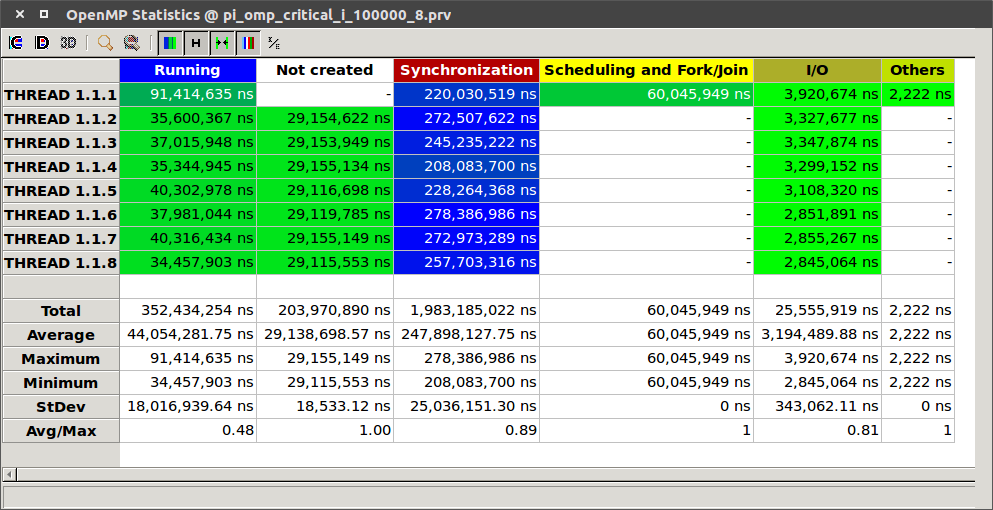
\includegraphics[width=\textwidth]{images/image02}
    \caption{Profile with 1 thread}
    \label{fig:image02}
\end{figure}

\begin{figure}[H]
    \centering
    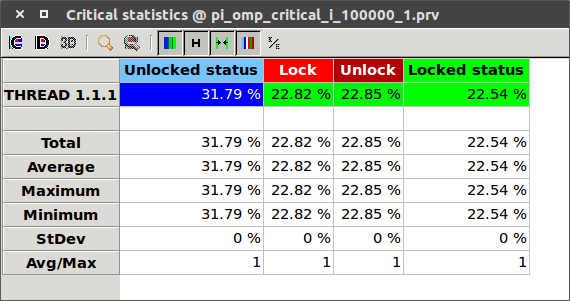
\includegraphics[width=0.7\textwidth]{images/image03}
    \caption{Profile with 8 threads}
    \label{fig:image03}
\end{figure}

\autoref{fig:image02} and \autoref{fig:image03} let us see the amount of time lost in synchronization compared to the running time. The relationship between the synchronization time and the running time with one thread is about 92\% compared with 8 threads about 563\% which show us where is a big part of the overhead.

Another reason for the overhead is the scheduling and Fork/Join region than for making the same task with one thread is 1820 times faster than with 8 threads.

\begin{enumerate}[resume]
	\item \textbf{Which is the order of magnitude for the overhead associated with the execution of \texttt{atomic} memory accesses in \texttt{OpenMP}? How and why does the overhead associated with \texttt{atomic} increase with the number of processors? Reason the answers based on the execution times reported by the \texttt{pi\_omp.c} and \texttt{pi\_omp\_atomic.} programs.}
\end{enumerate}

\begin{table}[H]
    \centering
    \begin{tabular}{l|rrrrr}
        \parbox{2.7cm}{100.000.000\\ iterations time (s)} &  \verb|paralel| & \verb|atomic| & Overheads & Overhead \% & \parbox{2cm}{\raggedleft Overhead per thread} \\
        \hline
        1 thread & 0,85 & 1,45 & 0,60 & 41\% & 0,90 \\
        8 threads & 0,12 & 10,96 & 10,84 & 99\% & 1,36
    \end{tabular}
\end{table}

The order of magnitude is about 1 s per thread per 100 000 000 iterations. 

The overhead time is increasing more than linary cause the overhead per thread increased when the number of processor increased. That’s caused by synchronization among threads.

\begin{enumerate}[resume]
	\item \textbf{In the presence of false sharing (as it happens in \texttt{pi\_omp\_sumvector.c}), which is the additional average time for each individual access to memory that you observe? What is causing this increase in the memory access time? Reason the answers based on the execution times reported by the \texttt{pi\_omp\_sumvector.c} and \texttt{pi\_omp\_padding.c} programs. Explain how padding is done in \texttt{pi\_omp\_padding.c}.}
\end{enumerate}

This are the timings by 100.000 accesses:
\begin{itemize}
	\item \verb|pi_omp_sumvector.c|: 33.392.181ns
	\item \verb|pi_omp_padding.c|: 39.000.423ns
\end{itemize}

The difference is 5.608.242ns which is about 56,082 ns of additional average time for each individual access to memory. This increase of access time can be caused by multiple cache misses because any cache level (neither level 3) will have the data cached which this implies reading 8 times (one for each thread) directly to the main memory.

The padding is done by creating a \verb|sumvector| bigger than needed, this vector contains one block of the cache size to allow the thread to have its own block of the vector. This can bee seen in the following line:

\begin{lstlisting}[language=C]
double sumvector[NUMTHRDS][CACHE_SIZE/sizeof(double)];
\end{lstlisting}


\begin{enumerate}[resume]
	\item \textbf{ Complete the following table with the execution times of the different versions for the computation of Pi that we provide to you in this first laboratory assignment when executed with 100.000.000 iterations. The speed–up has to be computed with respect to the execution of the serial version. For each version and number of threads, how many executions have you performed? }
\end{enumerate}

\begin{table}[H]
	\centering
	\begin{tabular}{l|rrr}
		\textbf{Version} & \textbf{1 processor} & \textbf{8 processors} & \textbf{speed-up} \\
		\hline
		\verb|pi_seq.c| & 0,79  & - & 1 \\
		\verb|pi_omp.c| (sumlocal) & 0,79 & 0,21 & 3,72  \\
		\verb|pi_omp_critical.c| & 1,83 & 22,94 & 0,08  \\
		\verb|pi_omp_lock.c| & 1,79 & 4,15 & 0,43  \\
		\verb|pi_omp_atomic.c| & 1,44 & 8,16 & 0,18  \\
		\verb|pi_omp_sumvector.c| & 0,79 & 0,65 & 1,21  \\
		\verb|pi_omp_padding.c| & 0,79 & 0,12 & 6,51  \\
	\end{tabular}
\end{table}

To make this tests two executions have been performed.

\end{document}